\begin{figure}
    \centering
\begin{knitrout}
\definecolor{shadecolor}{rgb}{0.969, 0.969, 0.969}\color{fgcolor}
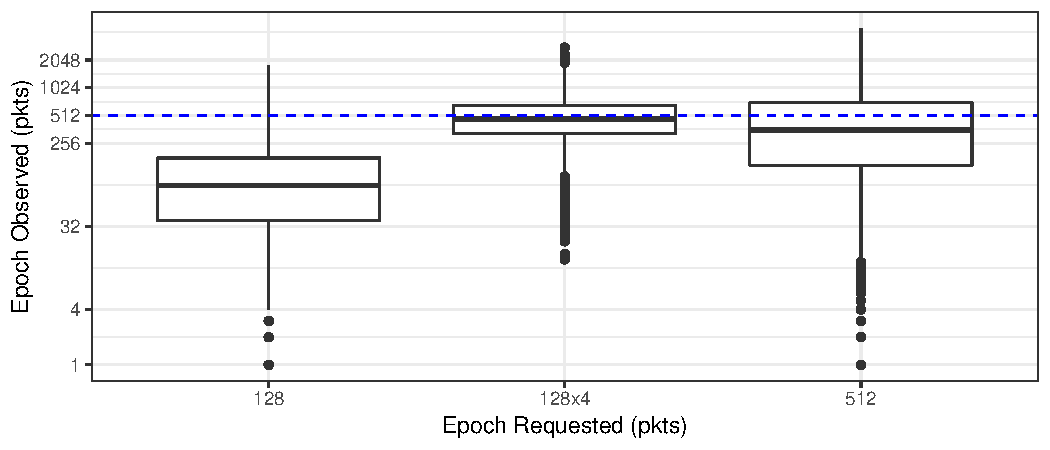
\includegraphics[width=\maxwidth]{figure/micro:epoch-1} 

\end{knitrout}
    \caption{Distribution of observed epoch sizes based on the desired epoch size. Suppose we
    need an epoch size of 512. By setting the epoch size to $\frac{1}{4}$ of that and using
    a sliding window over the last 4 epochs, we can achieve the same average epoch size with
    significantly lower variance than if we were to set the epoch size to 512 directly.
    \fc{todo: real eval data}}
    \label{fig:micro:epoch}
\end{figure}
